\documentclass[10pt,twocolumn,letterpaper]{article}

\usepackage{cvpr}
\usepackage{times}
\usepackage{epsfig}
\usepackage{graphicx}
\usepackage{amsmath}
\usepackage{amssymb}
\usepackage{textcomp}

\usepackage{eqnarray}
\usepackage{amsmath}
\usepackage{units}
\usepackage{graphicx}
\usepackage{caption}
\usepackage{subcaption}
\usepackage{url}
\usepackage{algorithmicx}
\usepackage{algpseudocode}
\usepackage{mathtools}
\usepackage{bbm}
\usepackage{stackengine}
\usepackage{xfrac}

\usepackage{multirow}
\usepackage{colortbl}

\allowdisplaybreaks

\DeclarePairedDelimiter{\abs}{\lvert}{\rvert}
\DeclarePairedDelimiter{\norm}{\lVert}{\rVert}
\DeclareMathOperator{\atantwo}{atan2}
\DeclareMathOperator{\diag}{diag}
\DeclareMathOperator*{\argmin}{arg\,min}

\definecolor{Yellow}{rgb}{1,1, 0.6}
\definecolor{Red}{rgb}{1, 0.6, 0.6}

\newcommand{\todo}[1] {{\color{red}[#1]}}
\newcommand{\floor}[1]{\left \lfloor #1 \right \rfloor}
\newcommand{\binwidth}{h}
\newcommand{\E}[1]{\operatorname{E}\left\lbrack#1\right\rbrack}
\newcommand{\fftv}[1]{\mathcal{F}_\mathrm{v} \left( #1 \right)}
\newcommand{\ifftv}[1]{\mathcal{F}^{-1}_\mathrm{v} \left( #1 \right)}
\newcommand{\fft}[1]{\mathcal{F}\left( #1 \right )}
\newcommand{\ifft}[1]{\mathcal{F}^{-1}\left( #1 \right )}
\newcommand{\lossreg}[1]{\mathrm{loss_{reg}}\left( #1 \right )}
\newcommand{\lossdata}[1]{f\left( #1 \right )}
% \newcommand{\lossdata}[1]{\mathrm{loss}\left( #1 \right )}
\DeclareMathOperator*{\argmax}{arg\,max}

\newcommand{\sixwidth}{1.11in}
\newcommand{\threewidth}{2.22in}

\def\lf{\left\lfloor}
\def\rf{\right\rfloor}

\usepackage{expl3}
\ExplSyntaxOn
\newcommand\latinabbrev[1]{
  \peek_meaning:NTF . {% Same as \@ifnextchar
    #1\@}%
  { \peek_catcode:NTF a {% Check whether next char has same catcode as \'a, i.e., is a letter
      #1.\@ }%
    {#1.\@}}}
\ExplSyntaxOff
\def\etal{\latinabbrev{et al}}

% Include other packages here, before hyperref.

\usepackage[breaklinks=true,bookmarks=false]{hyperref}

\cvprfinalcopy % *** Uncomment this line for the final submission

\def\cvprPaperID{287} % *** Enter the CVPR Paper ID here
\def\httilde{\mbox{\tt\raisebox{-.5ex}{\symbol{126}}}}

% Pages are numbered in submission mode, and unnumbered in camera-ready
\ifcvprfinal\pagestyle{empty}\fi
\begin{document}

\title{Fast Fourier Color Constancy \\ Supplement}

\author{
Jonathan T. Barron\\
{\tt\small barron@google.com}
\and
Yun-Ta Tsai\\
{\tt\small yuntatsai@google.com}
}
\maketitle


\section{Pretraining}

In the paper we described the data term for our loss function $f(\cdot)$ which
takes a toroidal PDF $P(i,j)$, fits a bivariate von Mises
distribution to $P$, and then computes the negative log-likelihood
of the true white point $L^*$ under that distribution.
This loss is non-convex, and therefore may behave erratically
in the earliest training iterations. This issue is compounded by our
differentiable BVM fitting procedure, which may be inacurate when $P$ has
a low concentration, which is often the case in early iterations.
For this reason, we train our model in two stages:
In the ``pretraining'' stage we replace the data term in our loss function
with a more simple loss: straightforward logistic regression with respect to
$P$ and some ground-truth PDF $P^*$ (Eq.~\ref{eq:losspre}), and then
in the second training stage we use the data term described in the paper while
using the output of pretraining to initialize the model.
Because our regularization is also convex, using this pretraining loss makes
our entire optimization problem convex and therefore straightforward to
optimize, and (when coupled with our use of LBFGS for optimization instead
of some SGD-like approach) also makes training deterministic.

Computing a logistic loss is straightforward: we compute a ground-truth PDF
$P^*$ from the ground-truth illuminant $L^*$, and then compute a standard
logistic loss.
\begin{align}
P^*(i,j) =& \operatorname{mod} \left( { L_u^* - u_\mathit{lo} \over \binwidth} - i, n \right) < 1 \\
\wedge& \operatorname{mod} \left( { L_v^* - v_\mathit{lo} \over \binwidth} - j, n \right) < 1 \nonumber \\
f_{\mathrm{pretrain}}(P) &= -\sum_{i,j} P^*(i,j) \log(P(i,j)) \label{eq:losspre}
\end{align}
This loss behaves very similarly to the loss used in CCC \cite{BarronICCV2015},
but it has the added benefit of being convex.

\section{Backpropagation}

The bivariate von Mises estimation procedure described in the paper can be
thought of as a ``layer'' in a deep learning architecture, as our end-to-end
training procedure requires that we be able to backpropagate through the fitting
procedure and the loss computation. Here we present the gradients of the critical
equations described in the paper.

\newcommand{\ishift}{\bar{i}}
\newcommand{\jshift}{\bar{j}}

\begin{equation}
\nabla_{\boldsymbol{\mu}} \lossdata{\boldsymbol{\mu}, \boldsymbol{\Sigma}} = -2 \boldsymbol{\Sigma}^{-1} \left( \begin{bmatrix}
L^*_u \\ L^*_v
\end{bmatrix} - \boldsymbol{\mu} \right)
\end{equation}
\begin{equation}
\resizebox{3.25in}{!}{$
\nabla_{\boldsymbol{\Sigma}} \lossdata{\boldsymbol{\mu}, \boldsymbol{\Sigma}}  = \boldsymbol{\Sigma}^{-1} - \boldsymbol{\Sigma}^{-1} \left( \begin{bmatrix}
L^*_u \\ L^*_v
\end{bmatrix} - \boldsymbol{\mu} \right) \left( \begin{bmatrix}
L^*_u \\ L^*_v
\end{bmatrix} - \boldsymbol{\mu} \right)^\mathrm{T} \boldsymbol{\Sigma}^{-1} \nonumber
$}
\end{equation}
\begin{equation}
\nabla_{P(i,j)}\boldsymbol{\mu} =
\left({n \binwidth \over 2\pi}\right) \begin{bmatrix}
{x_i \sin(\theta(i)) - y_i \cos(\theta(i)) \over x_i^2 + y_i^2} \\
{x_j \sin(\theta(j)) - y_j \cos(\theta(j)) \over x_j^2 + y_j^2}
\end{bmatrix}
\end{equation}
\begin{equation}
\resizebox{3.25in}{!}{$
\nabla_{P(i,j)}\boldsymbol{\Sigma} = h^2 \begin{bmatrix}
\ishift \left( \ishift - 2\E{\ishift} \right), \quad
\left( \ishift - \E{\ishift} \right) \left( \jshift - \E{\jshift} \right) - \E{\ishift}\E{\jshift} \\
\left( \ishift - \E{\ishift} \right) \left( \jshift - \E{\jshift} \right) - \E{\ishift}\E{\jshift}, \quad
\jshift \left( \jshift - 2\E{\jshift} \right) \nonumber
\end{bmatrix}
$}
\end{equation}
By chaining these gradients together we can backpropagate the gradient of the loss
back onto the input PDF $P$. Backpropagating through the softmax operation and the convolution
(and illumination gain/bias) is straightforward and so is not detailed here.

\section{Deep Models}

In the main paper we stated that Models N, O, and P use an alternative parametrization
to incorporate external features during training and testing.
%
This parameterization allows our model to reason about things other than
simple pixel and edge log-chroma histograms, like semantics and camera metadata.
%
In the basic model presented in the main paper, we learn a set of weights
$( \{F_k \}, G, B )$, where these weights determine the shape of the filters
used during convolution and the per-color gain/bias applied to the output of
that convolution.
%
Let us abstractly refer to the concatenation of these (preconditioned,
Fourier-domain) weights as $\mathbf{w}$, and let the loss contributed by the data term
for training data instance $i$ be $f_i(\mathbf{w})$
(here $f_i(\mathbf{w})$ does not just apply a loss, but first undoes the
preconditioning transformation and maps from our real FFT vector space to a
complex 2D FFT).
%
Training our basic model can be thought of as simply finding
\begin{equation}
\argmin_{\mathbf{w}} \sum_i f_i \left( \mathbf{w} \right)
\end{equation}
%
To generalize our model, instead of learning a single model $\mathbf{w}$, we
instead define a feature vector for each training instance $\mathbf{x}_i$
and learn a mapping from each $\mathbf{x}_i$ to some $\mathbf{w}_i$ such that
the loss for all $\{ \mathbf{w}_i \}$ is minimized.
%
Instead of learning a single $\mathbf{w}$, we learn the weights in a small
$2$-layer neural network with a ReLU activation function, where those
network weights define the mapping from features to FFCC parameters.
%
The resulting optimization problem during training is:
\begin{equation}
\argmin_{\mathbf{W}_1, \mathbf{b}_1, \mathbf{W}_2, \mathbf{b}_2} \sum_i f_i \left( \mathbf{W}_2 \max(0, \mathbf{W}_1 \mathbf{x}_i + \mathbf{b}_1) + \mathbf{b}_2 \right)
\end{equation}
Like in all other experiments we train using batch L-BFGS, but instead of the
two-stage training used in the shallow model (a convex ``pretraining''
loss and a nonconvex final loss), we have only one training stage:
$64$ iterations of LBFGS, in which we minimize a weighted sum of the two losses.
%
Our input vectors $\{ \mathbf{x}_i \}$ are whitened before training, and
the whitening transformation is absorbed into $\mathbf{W}_1$ and $\mathbf{b}_1$
after training so that unwhitened features can be used at test-time.
%
Our weights are initialized to random Gaussian noise, unlike the shallow model
which is initialized to all zeros.
%
Unlike our ``shallow'' model, in which $\mathbf{w}$ is regularized during training,
for our ``deep'' models we do not directly regularize each $\mathbf{w}_i$ but instead
indirectly regularize all $\mathbf{w}_i$ by minimizing the squared 2-norm of each $\mathbf{W}_i$ and $\mathbf{b}_i$.
%
This use of weight decay to regularize our model depends critically on the
frequency-domain preconditioning we use, which causes a simple weight decay to
indirectly impose the careful smoothness regularizer that was constructed for our shallow model.
%
Note that our ``deep'' model is equivalent to our ``shallow'' model if the input vector is empty
(ie, $\mathbf{x}_i = [\,]$), as $\mathbf{b}_2$ would behave equivalently to $\mathbf{w}$ in that case.
%
We use $4$ hidden units for Models N and O, and $8$ hidden units for Model P
(which uses the concatenated features from both Models N and O).
%
The magnitude of the noise used for initialization and of the weight decay for
each layer of the network are tuned using cross-validation.

To produce the ``metadata'' features used in Models O and P we use the EXIF tags
included in the Gehler-Shi dataset.
%
Using external information in this way is unusual in the color constancy
literature, which is why this aspect of our model is relegated to just two
experiments (all figures and other results do not use external metadata).
%
In contrast, camera manufacturers spend significant effort considering sensor
spectral properties and other sources of information that may be useful when
building a white balance system.
%
For example, knowing that two images came from two different sensors (as is the
case in the Gehler-Shi dataset) allows for a more careful treatment of absolute
color and black body radiation.
%
And knowing the absolute brightness of the scene (indicated by the camera's
exposure time, etc) can be a useful cue for distinguishing between the bright
light of the sun and the relatively low light of man made light sources.
%
As the improved performance of Model O demonstrates, this other information is
indeed informative and can induce a significant reduction in error.
%
We use a compact feature vector that encodes the outer product of the
exposure settings of the camera and the name of the camera sensor itself, all
extracted from the EXIF tags included in the public dataset:
\begin{align}
\mathbf{x}_i =&  \mathrm {vec} ( \\
& [\log(\mathrm{shutter\_speed}_i); \log(\mathrm{f\_number}_i); 1] \nonumber \\
\times & [\mathbf {1}_{\mathrm{Canon1D}} (\mathrm{camera}_i), \mathbf {1}_{\mathrm{Canon5D}} (\mathrm{camera}_i), 1]) \nonumber
\end{align}
Note that the Gehler-Shi dataset uses images from two different Canon cameras,
as reflected here.
%
The log of the shutter speed and F number are chosen as features because,
in theory, their difference should be proportional to the log of the exposure
value of the image, which should indicate the amount of light receiving by the
camera sensor.

The ``semantics'' features used in Models N and P are simply the output of the
CNN model used in \cite{Wang2014}, which was run on the pre-whitebalance image
after it is center-cropped to a square and resized to $256 \times 256$.
%
Because this image is in the sensor colorspace, before passing it to the CNN
we scale the green channel by $0.6$, apply a CCM, and apply an sRGB gamma
curve.
%
These semantic features have a modest positive effect.

\section{Real Bijective FFT}

In the paper we describe $\fftv{Z}$, a FFT variant
that takes the 2D FFT of a $n \times n$ real-valued 2D image $Z$ and then
linearizes it into a real-valued vector with no redundant values.
Having this FFT-like one-to-one mapping between real 2D images and real 1D vectors
enables our frequency-domain preconditioner.

Our modified FFT function is defined as:
\begin{align}
\fftv{Z} &= \left[ \begin{array}{l}
\operatorname {Re} (\fft{Z}(0 : \nicefrac{n}{2}, 0)) \\
\operatorname {Re} (\fft{Z}(0 : \nicefrac{n}{2}, \nicefrac{n}{2})) \\
\operatorname {Re} (\fft{Z}(0 : (n-1), 1:(\nicefrac{n}{2}-1))) \\
\operatorname {Im} (\fft{Z}(1 : (\nicefrac{n}{2}-1), 0)) \\
\operatorname {Im} (\fft{Z}(1 : (\nicefrac{n}{2}-1), \nicefrac{n}{2}-1)) \\
\operatorname {Im} (\fft{Z}(0 : (n-1), 1:(\nicefrac{n}{2}-1))) \\
\end{array} \right]
\end{align}
Where $\fft{Z}(i, j)$ is the complex number at the zero-indexed $(i,j)$
position in the FFT of $Z$, and
 $\operatorname {Re}(\cdot)$ and
$\operatorname {Im}(\cdot)$ extract real and imaginary components, respectively.
The output of $\fftv{Z}$ is an $n^2$-dimensional vector, as it must be for our
mapping to preserve all FFT coefficients with no redundancy.
To preserve the scale of the FFT through this mapping we scale $\fftv{Z}$ by
$\sqrt{2}$, ignoring the entries that correspond to:
\begin{align}
&\operatorname {Re}(\fft{Z}(0, 0)) \nonumber \\
&\operatorname {Re}(\fft{Z}(0, \nicefrac{n}{2})) \nonumber \\
&\operatorname {Re}(\fft{Z}(\nicefrac{n}{2}, 0)) \nonumber \\
&\operatorname {Re}(\fft{Z}(\nicefrac{n}{2}, \nicefrac{n}{2}))
\end{align}
This scaling ensure that the magnitude of $Z$ is preserved:
\begin{equation}
\norm{\fftv{Z}}^2 = \abs{\fft{Z}}^2
\end{equation}
To compute the inverse of $\fftv{\cdot}$ we
undo this scaling,
undo the vectorization by filling in a subset of the elements of
$\fft{Z}$ from the vector representation,
set the other elements of $\fft{Z}$ such that Hermitian symmetry holds,
and the invert the FFT.

\section{Results}

Because our model produces a complete posterior distribution over illuminants
in the form of a covariance matrix $\boldsymbol{\Sigma}$, each of our
illuminant estimates comes with a measure of confidence in the form
of the entropy: ${1 \over 2} \log{|\boldsymbol{\Sigma}| }$ (ignoring a constant shift).
A low entropy suggests a tight concentration of the output distribution, which
tends to be well-correlated with a low error.
To demonstrate this we present a novel error metric, which is twice the area
under the curve formed by ordering all images
(the union of all test-set images from each cross-validation fold)
by ascending entropy and normalizing by the number of images.
In Figure~\ref{fig:confidence_err} we visualize this error metric and show
that our entropy-ordered error is substantially lower than the mean error
for both of our datasets, which shows that a low entropy is suggestive
of a low error.
We are not aware of any other color constancy technique which explicitly
predicts a confidence measure, and so we do not compare against any
existing technique, but it can be demonstrated that if the entropy used
to sort error is decorrelated with error (or, equivalently, if the error cannot
be sorted due to the lack of the means to sort it)
that entropy-ordered error will on average be equal to mean error.

To allow for a better understanding of our model's performance, we present
images from the Gehler-Shi dataset \cite{Gehler08,shifunt}
(Figures~\ref{fig:results1}-\ref{fig:results10})
and the Canon 1Ds MkIII camera from the Cheng \etal\, dataset \cite{Cheng14}
(Figures~\ref{fig:results11}-\ref{fig:results15}).
There results were produced using Model J presented in the main paper.
For each dataset we perform three-fold cross validation, and with that we produce
output predictions for each image along with an error measure (angular RGB
error) and an entropy measure (the entropy of the covariance matrix of our
predicted posterior distribution over illuminants). The images chosen here were
selected by sorting images from each dataset by increasing error and evenly sampling
images according to that ordering (10 from Gehler-Shi, 5 from the smaller Cheng
dataset).
This means that the first image in each sequence is the lowest error image,
and the last is the highest.
The rendered images include the color checker used in creating the ground-truth
illuminants used during training, but it should be noted that these color checkers
are masked out when these images are used during training and evaluation.
For each image we present: a) the input image, b) the predicted bivariate von Mises
distribution over illuminants, c) our estimated illuminant and white-balanced
image (produced by dividing the estimated illuminant into the input image),
and d) the ground-truth illuminant and white-balanced image.
Our log-chroma histograms are visualized using gray light de-aliasing
to assign each $(i,j)$ coordinate a color,
with a blue dot indicating the location/color of the ground-truth illuminant,
a red dot indicating our predicted illuminant $\boldsymbol{\mu}$
and a red ellipse indicating the predicted covariance of the illuminant $\boldsymbol{\Sigma}$.
The bright lines in the histogram indicate the locations where $u=0$ or $v=0$.
The reported entropy of the covariance $\boldsymbol{\Sigma}$ corresponds to the
spread of the covariance (low entropy = small spread).
We see that our low error predictions tend to
have lower entropies, and vice versa, confirming our analysis in
Figure~\ref{fig:confidence_err}.
We also see that the ground-truth
illuminant tends to lie within the estimated covariance matrix, though not
always for the largest-error images.

\begin{figure}[!]
\centering
  \begin{subfigure}[!]{1.55in}
    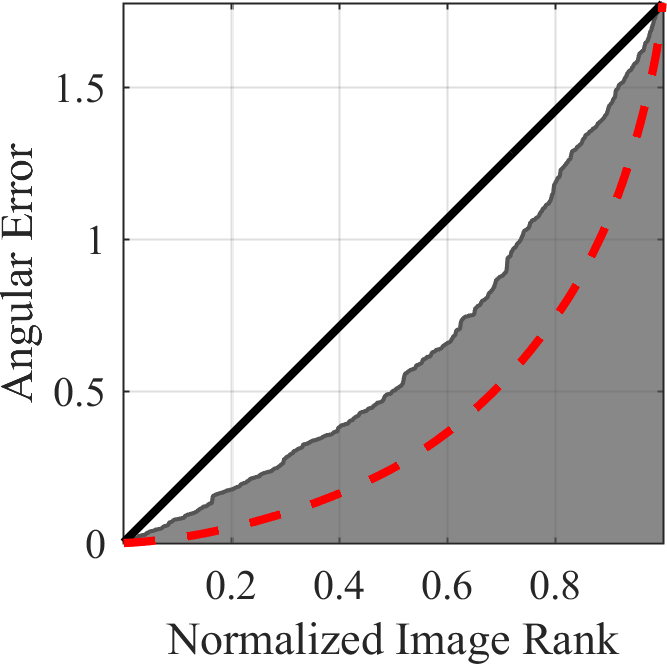
\includegraphics[width=1.5in]{figures/confidence_err_gehler.png}
    \caption{Gehler-Shi dataset \cite{Gehler08,shifunt}}
  \end{subfigure}
  \hspace{0.05in}
  \begin{subfigure}[!]{1.55in}
    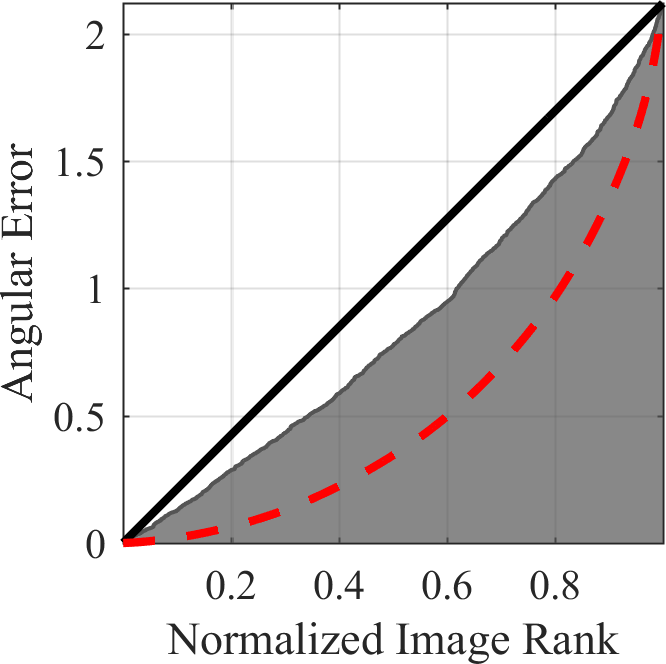
\includegraphics[width=1.5in]{figures/confidence_err_cheng.png}
    \caption{Cheng \etal\, dataset \cite{Cheng14}}
  \end{subfigure}
  \small
  \begin{tabular}{ r@{}c r r}
  EO Error: \quad\, & 1.287 & \hspace{1.0in} 1.696 & \hspace{0.5in}\\
  Mean Error: \quad\, & 1.775 & \hspace{1.0in} 2.121  & \hspace{0.5in}
  \end{tabular}
  \caption{
    By sorting each image by the entropy of its posterior distribution we
    can show that entropy correlates with error.
    Here we sort the images by ascending entropy and plot the cumulative sum of the error,
    filling in the area under that curve with gray.
    If entropy was not correlated with error we would expect the area under the
    curve to match the black line, and if entropy was perfectly correlated with
    error then the area under the curve would exactly match the dashed red line.
    We report twice the area under the curve as ``entropy-ordered'' error
    (mean error happens to be twice the area under the diagonal line).
    \label{fig:confidence_err}
  }
\end{figure}

In Figure~\ref{fig:realimages} we visualize a set of images taken from a Nexus
6 in the HDR+ mode \cite{Hasinoff2016} after being white-balanced by
Model Q in the main paper (the version designed to run on thumbnail images).


\section{Color Rendering}

All images are rendered by
applying the RGB gains implied by the estimated illuminant, applying some
color correction matrix (CCM)
and then applying an sRGB gamma-correction function (the
$C_{\mathrm{linear}}$ to $C_{\mathrm {srgb}}$ mapping in
\url{http://en.wikipedia.org/wiki/SRGB}).
For each camera in the datasets we use we estimate our own CCMs using the imagery,
which we present here.
These CCMs do not affect our illuminant estimation or our results,
and are only relevant to our visualizations.
Each CCM is estimated through an iterative least-squares process in which
we alternatingly:
1) estimate the ground-truth RGB gains for each image from a camera
by solving a least-squares system using our current CCM, and
2) use our current gains to estimate a row-normalized CCM using a constrained
least-squares solve.
Our estimated ground-truth gains are not used in this paper.
For the ground-truth sRGB colors of the Macbeth color chart we use the hex values
provided here: \url{http://en.wikipedia.org/wiki/ColorChecker#Colors}
which we linearize.

\begin{align}
\small{\mathrm{GehlerShi, Canon1D}}
\begin{bmatrix}
\phantom{-}2.2310 & -1.5926 & \phantom{-}0.3616 \\
-0.1494 & \phantom{-}1.4544 & -0.3050 \\
\phantom{-}0.1641 & -0.6588 & \phantom{-}1.4947 \\
\end{bmatrix} \nonumber
 \\
\small{\mathrm{GehlerShi, Canon5D}}
\begin{bmatrix}
\phantom{-}1.7494 & -0.8470 & \phantom{-}0.0976 \\
-0.1565 & \phantom{-}1.4380 & -0.2815 \\
\phantom{-}0.0786 & -0.5070 & \phantom{-}1.4284 \\
\end{bmatrix} \nonumber
\\
\small{\mathrm{Cheng, Canon1DsMkIII}}
\begin{bmatrix}
\phantom{-}1.7247 & -0.7791 & \phantom{-}0.0544 \\
-0.1436 & \phantom{-}1.4632 & -0.3195 \\
\phantom{-}0.0589 & -0.4625 & \phantom{-}1.4037 \\
\end{bmatrix} \nonumber
 \\
\small{\mathrm{Cheng, Canon600D}}
\begin{bmatrix}
\phantom{-}1.8988 & -0.9897 & \phantom{-}0.0909 \\
-0.2058 & \phantom{-}1.6396 & -0.4338 \\
\phantom{-}0.0749 & -0.7030 & \phantom{-}1.6281 \\
\end{bmatrix} \nonumber
 \\
\small{\mathrm{Cheng, FujifilmXM1}}
\begin{bmatrix}
\phantom{-}1.4183 & -0.2497 & -0.1686 \\
-0.2230 & \phantom{-}1.6449 & -0.4219 \\
\phantom{-}0.0785 & -0.5980 & \phantom{-}1.5195 \\
\end{bmatrix} \nonumber
 \\
\small{\mathrm{Cheng, NikonD5200}}
\begin{bmatrix}
\phantom{-}1.3792 & -0.3134 & -0.0659 \\
-0.0826 & \phantom{-}1.3759 & -0.2932 \\
\phantom{-}0.0483 & -0.4553 & \phantom{-}1.4070 \\
\end{bmatrix} \nonumber
 \\
\small{\mathrm{Cheng, OlympusEPL6}}
\begin{bmatrix}
\phantom{-}1.6565 & -0.4971 & -0.1595 \\
-0.3335 & \phantom{-}1.7772 & -0.4437 \\
\phantom{-}0.0895 & -0.7023 & \phantom{-}1.6128 \\
\end{bmatrix} \nonumber
 \\
\small{\mathrm{Cheng, PanasonicGX1}}
\begin{bmatrix}
\phantom{-}1.5629 & -0.5117 & -0.0512 \\
-0.2472 & \phantom{-}1.7590 & -0.5117 \\
\phantom{-}0.1395 & -0.8945 & \phantom{-}1.7550 \\
\end{bmatrix} \nonumber
 \\
\small{\mathrm{Cheng, SamsungNX2000}}
\begin{bmatrix}
\phantom{-}1.5770 & -0.4351 & -0.1419 \\
-0.1747 & \phantom{-}1.5225 & -0.3477 \\
\phantom{-}0.0573 & -0.6397 & \phantom{-}1.5825 \\
\end{bmatrix} \nonumber
 \\
\small{\mathrm{Cheng, SonyA57}}
\begin{bmatrix}
\phantom{-}1.5963 & -0.5545 & -0.0418 \\
-0.1343 & \phantom{-}1.5331 & -0.3988 \\
\phantom{-}0.0563 & -0.4026 & \phantom{-}1.3463 \\
\end{bmatrix} \nonumber
\end{align}


\begin{figure*}[!]
\centering
  \begin{subfigure}[!]{1.7in}
    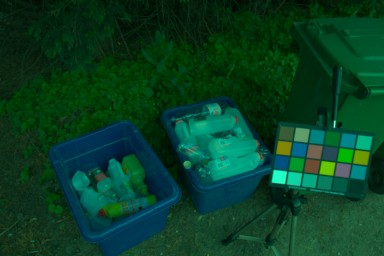
\includegraphics[width=1.6in]{figures/results/gehlershi/00000300_input.jpg}
    \caption{\footnotesize Input Image}
  \end{subfigure}
  \begin{subfigure}[!]{1.17in}
    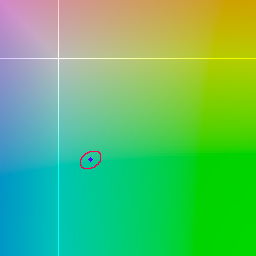
\includegraphics[width=1.07in]{figures/results/gehlershi/00000300_chroma.png}
    \caption{\footnotesize Illuminant Posterior}
  \end{subfigure}
\begin{subfigure}[!]{1.9in}
    
\includegraphics[width=0.133in]{figures/results/gehlershi/00000300_illum.png}\!
    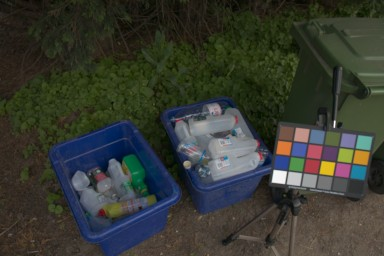
\includegraphics[width=1.6in]{figures/results/gehlershi/00000300_prediction.jpg}
    \caption{\footnotesize Our prediction}
  \end{subfigure}
  \begin{subfigure}[!]{1.9in}
    
\includegraphics[width=0.133in]{figures/results/gehlershi/00000300_illum_true.png}\!
    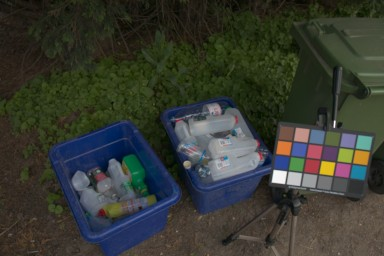
\includegraphics[width=1.6in]{figures/results/gehlershi/00000300_true.jpg}
    \caption{\footnotesize Ground Truth}
  \end{subfigure}
  \caption{
    A result from the Gehler-Shi dataset using Model J. Error = $0.02$\textdegree, entropy = $-6.48$
    \label{fig:results1}
  }
\end{figure*}

\begin{figure*}[!]
\centering
  \begin{subfigure}[!]{1.7in}
    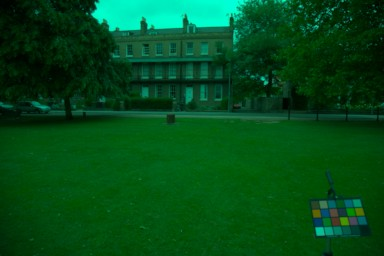
\includegraphics[width=1.6in]{figures/results/gehlershi/00000500_input.jpg}
    \caption{\footnotesize Input Image}
  \end{subfigure}
  \begin{subfigure}[!]{1.17in}
    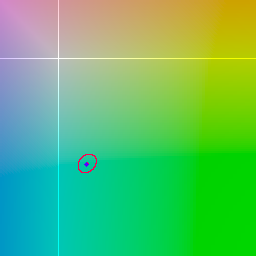
\includegraphics[width=1.07in]{figures/results/gehlershi/00000500_chroma.png}
    \caption{\footnotesize Illuminant Posterior}
  \end{subfigure}
\begin{subfigure}[!]{1.9in}
    
\includegraphics[width=0.133in]{figures/results/gehlershi/00000500_illum.png}\!
    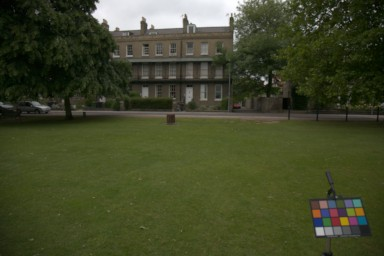
\includegraphics[width=1.6in]{figures/results/gehlershi/00000500_prediction.jpg}
    \caption{\footnotesize Our prediction}
  \end{subfigure}
  \begin{subfigure}[!]{1.9in}
    
\includegraphics[width=0.133in]{figures/results/gehlershi/00000500_illum_true.png}\!
    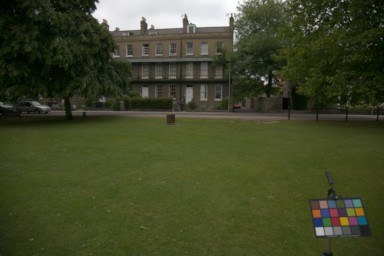
\includegraphics[width=1.6in]{figures/results/gehlershi/00000500_true.jpg}
    \caption{\footnotesize Ground Truth}
  \end{subfigure}
  \caption{
    A result from the Gehler-Shi dataset using Model J. Error = $0.26$\textdegree, entropy = $-6.55$
    \label{fig:results2}
  }
\end{figure*}


\begin{figure*}[!]
\centering
  \begin{subfigure}[!]{1.7in}
    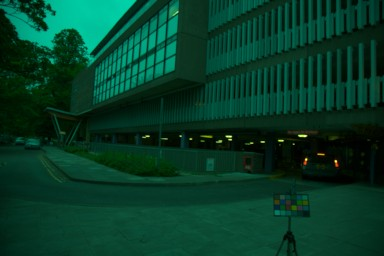
\includegraphics[width=1.6in]{figures/results/gehlershi/00000515_input.jpg}
    \caption{\footnotesize Input Image}
  \end{subfigure}
  \begin{subfigure}[!]{1.17in}
    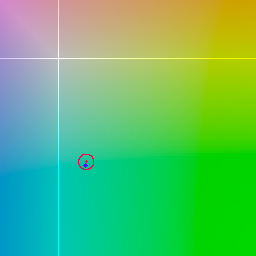
\includegraphics[width=1.07in]{figures/results/gehlershi/00000515_chroma.png}
    \caption{\footnotesize Illuminant Posterior}
  \end{subfigure}
\begin{subfigure}[!]{1.9in}
    
\includegraphics[width=0.133in]{figures/results/gehlershi/00000515_illum.png}\!
    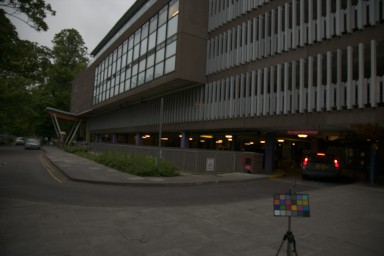
\includegraphics[width=1.6in]{figures/results/gehlershi/00000515_prediction.jpg}
    \caption{\footnotesize Our prediction}
  \end{subfigure}
  \begin{subfigure}[!]{1.9in}
    
\includegraphics[width=0.133in]{figures/results/gehlershi/00000515_illum_true.png}\!
    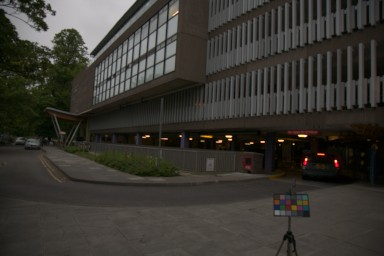
\includegraphics[width=1.6in]{figures/results/gehlershi/00000515_true.jpg}
    \caption{\footnotesize Ground Truth}
  \end{subfigure}
  \caption{
    A result from the Gehler-Shi dataset using Model J. Error = $0.46$\textdegree, entropy = $-6.91$
    \label{fig:results3}
  }
\end{figure*}


\begin{figure*}[!]
\centering
  \begin{subfigure}[!]{1.7in}
    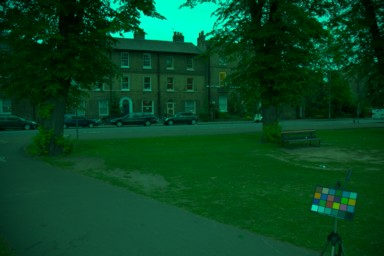
\includegraphics[width=1.6in]{figures/results/gehlershi/00000503_input.jpg}
    \caption{\footnotesize Input Image}
  \end{subfigure}
  \begin{subfigure}[!]{1.17in}
    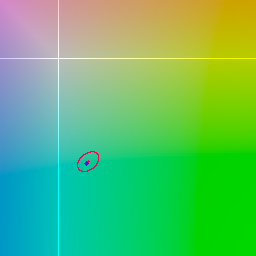
\includegraphics[width=1.07in]{figures/results/gehlershi/00000503_chroma.png}
    \caption{\footnotesize Illuminant Posterior}
  \end{subfigure}
\begin{subfigure}[!]{1.9in}
    
\includegraphics[width=0.133in]{figures/results/gehlershi/00000503_illum.png}\!
    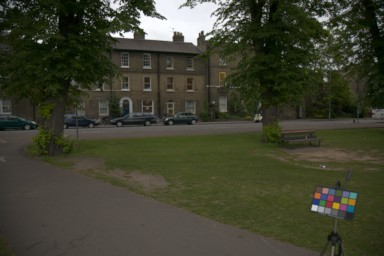
\includegraphics[width=1.6in]{figures/results/gehlershi/00000503_prediction.jpg}
    \caption{\footnotesize Our prediction}
  \end{subfigure}
  \begin{subfigure}[!]{1.9in}
    
\includegraphics[width=0.133in]{figures/results/gehlershi/00000503_illum_true.png}\!
    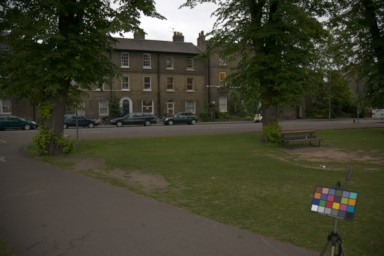
\includegraphics[width=1.6in]{figures/results/gehlershi/00000503_true.jpg}
    \caption{\footnotesize Ground Truth}
  \end{subfigure}
  \caption{
    A result from the Gehler-Shi dataset using Model J. Error = $0.63$\textdegree, entropy = $-6.37$
    \label{fig:results4}
  }
\end{figure*}


\begin{figure*}[!]
\centering
  \begin{subfigure}[!]{1.7in}
    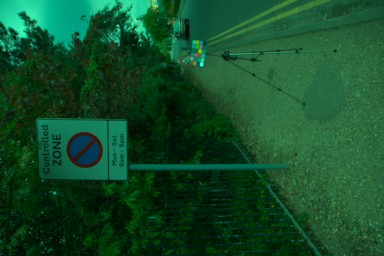
\includegraphics[width=1.6in]{figures/results/gehlershi/00000170_input.jpg}
    \caption{\footnotesize Input Image}
  \end{subfigure}
  \begin{subfigure}[!]{1.17in}
    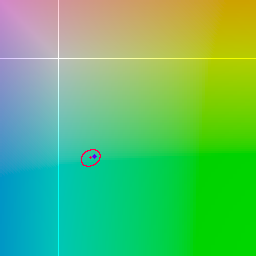
\includegraphics[width=1.07in]{figures/results/gehlershi/00000170_chroma.png}
    \caption{\footnotesize Illuminant Posterior}
  \end{subfigure}
\begin{subfigure}[!]{1.9in}
    
\includegraphics[width=0.133in]{figures/results/gehlershi/00000170_illum.png}\!
    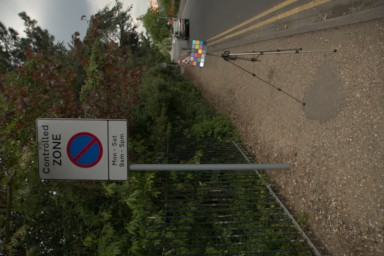
\includegraphics[width=1.6in]{figures/results/gehlershi/00000170_prediction.jpg}
    \caption{\footnotesize Our prediction}
  \end{subfigure}
  \begin{subfigure}[!]{1.9in}
    
\includegraphics[width=0.133in]{figures/results/gehlershi/00000170_illum_true.png}\!
    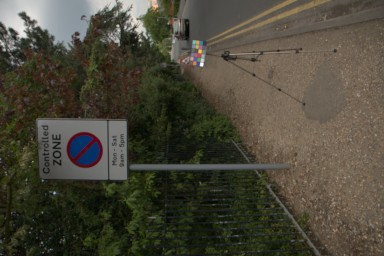
\includegraphics[width=1.6in]{figures/results/gehlershi/00000170_true.jpg}
    \caption{\footnotesize Ground Truth}
  \end{subfigure}
  \caption{
    A result from the Gehler-Shi dataset using Model J. Error = $0.83$\textdegree, entropy = $-6.62$
    \label{fig:results5}
  }
\end{figure*}

\begin{figure*}[!]
\centering
  \begin{subfigure}[!]{1.7in}
    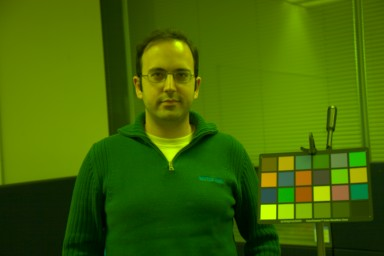
\includegraphics[width=1.6in]{figures/results/gehlershi/00000561_input.jpg}
    \caption{\footnotesize Input Image}
  \end{subfigure}
  \begin{subfigure}[!]{1.17in}
    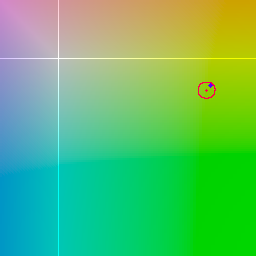
\includegraphics[width=1.07in]{figures/results/gehlershi/00000561_chroma.png}
    \caption{\footnotesize Illuminant Posterior}
  \end{subfigure}
\begin{subfigure}[!]{1.9in}
    
\includegraphics[width=0.133in]{figures/results/gehlershi/00000561_illum.png}\!
    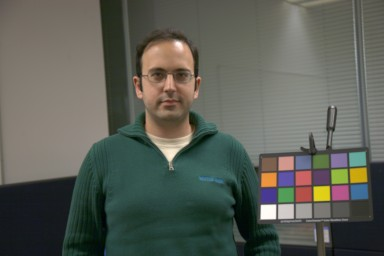
\includegraphics[width=1.6in]{figures/results/gehlershi/00000561_prediction.jpg}
    \caption{\footnotesize Our prediction}
  \end{subfigure}
  \begin{subfigure}[!]{1.9in}
    
\includegraphics[width=0.133in]{figures/results/gehlershi/00000561_illum_true.png}\!
    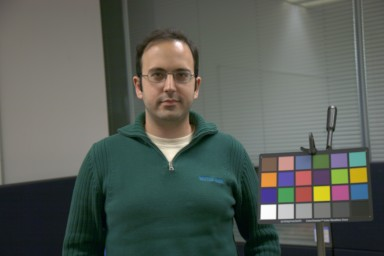
\includegraphics[width=1.6in]{figures/results/gehlershi/00000561_true.jpg}
    \caption{\footnotesize Ground Truth}
  \end{subfigure}
  \caption{
    A result from the Gehler-Shi dataset using Model J. Error = $1.19$\textdegree, entropy = $-6.71$
    \label{fig:results6}
  }
\end{figure*}

\begin{figure*}[!]
\centering
  \begin{subfigure}[!]{1.7in}
    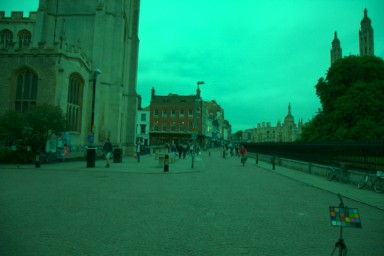
\includegraphics[width=1.6in]{figures/results/gehlershi/00000440_input.jpg}
    \caption{\footnotesize Input Image}
  \end{subfigure}
  \begin{subfigure}[!]{1.17in}
    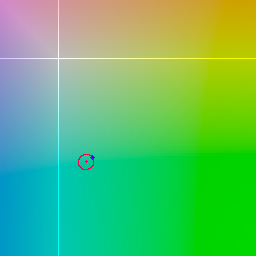
\includegraphics[width=1.07in]{figures/results/gehlershi/00000440_chroma.png}
    \caption{\footnotesize Illuminant Posterior}
  \end{subfigure}
\begin{subfigure}[!]{1.9in}
    
\includegraphics[width=0.133in]{figures/results/gehlershi/00000440_illum.png}\!
    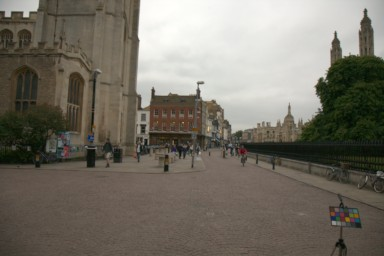
\includegraphics[width=1.6in]{figures/results/gehlershi/00000440_prediction.jpg}
    \caption{\footnotesize Our prediction}
  \end{subfigure}
  \begin{subfigure}[!]{1.9in}
    
\includegraphics[width=0.133in]{figures/results/gehlershi/00000440_illum_true.png}\!
    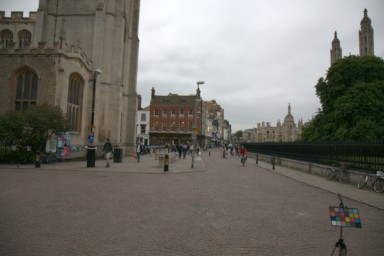
\includegraphics[width=1.6in]{figures/results/gehlershi/00000440_true.jpg}
    \caption{\footnotesize Ground Truth}
  \end{subfigure}
  \caption{
    A result from the Gehler-Shi dataset using Model J. Error = $1.61$\textdegree, entropy = $-6.88$
    \label{fig:results7}
  }
\end{figure*}


\begin{figure*}[!]
\centering
  \begin{subfigure}[!]{1.7in}
    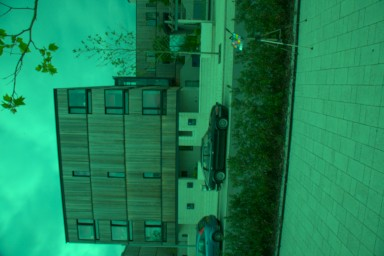
\includegraphics[width=1.6in]{figures/results/gehlershi/00000107_input.jpg}
    \caption{\footnotesize Input Image}
  \end{subfigure}
  \begin{subfigure}[!]{1.17in}
    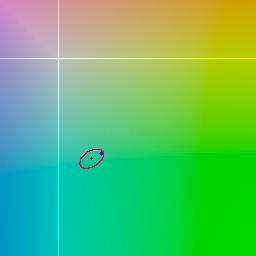
\includegraphics[width=1.07in]{figures/results/gehlershi/00000107_chroma.png}
    \caption{\footnotesize Illuminant Posterior}
  \end{subfigure}
\begin{subfigure}[!]{1.9in}
    
\includegraphics[width=0.133in]{figures/results/gehlershi/00000107_illum.png}\!
    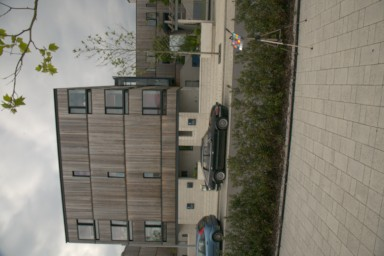
\includegraphics[width=1.6in]{figures/results/gehlershi/00000107_prediction.jpg}
    \caption{\footnotesize Our prediction}
  \end{subfigure}
  \begin{subfigure}[!]{1.9in}
    
\includegraphics[width=0.133in]{figures/results/gehlershi/00000107_illum_true.png}\!
    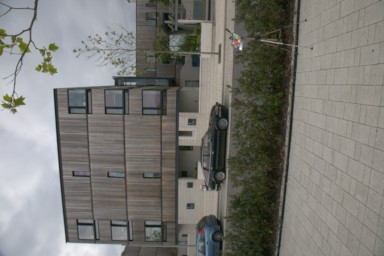
\includegraphics[width=1.6in]{figures/results/gehlershi/00000107_true.jpg}
    \caption{\footnotesize Ground Truth}
  \end{subfigure}
  \caption{
    A result from the Gehler-Shi dataset using Model J. Error = $2.35$\textdegree, entropy = $-6.32$
    \label{fig:results8}
  }
\end{figure*}


\begin{figure*}[!]
\centering
  \begin{subfigure}[!]{1.7in}
    \includegraphics[width=1.6in]{figures/results/gehlershi/00000524_input.jpg}
    \caption{\footnotesize Input Image}
  \end{subfigure}
  \begin{subfigure}[!]{1.17in}
    \includegraphics[width=1.07in]{figures/results/gehlershi/00000524_chroma.png}
    \caption{\footnotesize Illuminant Posterior}
  \end{subfigure}
\begin{subfigure}[!]{1.9in}
    \includegraphics[width=0.133in]{figures/results/gehlershi/00000524_illum.png}\!
    \includegraphics[width=1.6in]{figures/results/gehlershi/00000524_prediction.jpg}
    \caption{\footnotesize Our prediction}
  \end{subfigure}
  \begin{subfigure}[!]{1.9in}
    \includegraphics[width=0.133in]{figures/results/gehlershi/00000524_illum_true.png}\!
    \includegraphics[width=1.6in]{figures/results/gehlershi/00000524_true.jpg}
    \caption{\footnotesize Ground Truth}
  \end{subfigure}
  \caption{
    A result from the Gehler-Shi dataset using Model J. Error = $3.84$\textdegree, entropy = $-5.28$
    \label{fig:results9}
  }
\end{figure*}


\begin{figure*}[!]
\centering
  \begin{subfigure}[!]{1.7in}
    \includegraphics[width=1.6in]{figures/results/gehlershi/00000047_input.jpg}
    \caption{\footnotesize Input Image}
  \end{subfigure}
  \begin{subfigure}[!]{1.17in}
    \includegraphics[width=1.07in]{figures/results/gehlershi/00000047_chroma.png}
    \caption{\footnotesize Illuminant Posterior}
  \end{subfigure}
\begin{subfigure}[!]{1.9in}
    \includegraphics[width=0.133in]{figures/results/gehlershi/00000047_illum.png}\!
    \includegraphics[width=1.6in]{figures/results/gehlershi/00000047_prediction.jpg}
    \caption{\footnotesize Our prediction}
  \end{subfigure}
  \begin{subfigure}[!]{1.9in}
    \includegraphics[width=0.133in]{figures/results/gehlershi/00000047_illum_true.png}\!
    \includegraphics[width=1.6in]{figures/results/gehlershi/00000047_true.jpg}
    \caption{\footnotesize Ground Truth}
  \end{subfigure}
  \caption{
    A result from the Gehler-Shi dataset using Model J. Error = $21.64$\textdegree, entropy = $-4.95$
    \label{fig:results10}
  }
\end{figure*}



\begin{figure*}[!]
\centering
  \begin{subfigure}[!]{1.7in}
    \includegraphics[width=1.6in]{figures/results/cheng/00000191_input.jpg}
    \caption{\footnotesize Input Image}
  \end{subfigure}
  \begin{subfigure}[!]{1.17in}
    \includegraphics[width=1.07in]{figures/results/cheng/00000191_chroma.png}
    \caption{\footnotesize Illuminant Posterior}
  \end{subfigure}
\begin{subfigure}[!]{1.9in}
    \includegraphics[width=0.133in]{figures/results/cheng/00000191_illum.png}\!
    \includegraphics[width=1.6in]{figures/results/cheng/00000191_prediction.jpg}
    \caption{\footnotesize Our prediction}
  \end{subfigure}
  \begin{subfigure}[!]{1.9in}
    \includegraphics[width=0.133in]{figures/results/cheng/00000191_illum_true.png}\!
    \includegraphics[width=1.6in]{figures/results/cheng/00000191_true.jpg}
    \caption{\footnotesize Ground Truth}
  \end{subfigure}
  \caption{
    A result from the Cheng dataset using Model J. Error = $0.12$\textdegree, entropy = $-6.82$
    \label{fig:results11}
  }
\end{figure*}


\begin{figure*}[!]
\centering
  \begin{subfigure}[!]{1.7in}
    \includegraphics[width=1.6in]{figures/results/cheng/00000122_input.jpg}
    \caption{\footnotesize Input Image}
  \end{subfigure}
  \begin{subfigure}[!]{1.17in}
    \includegraphics[width=1.07in]{figures/results/cheng/00000122_chroma.png}
    \caption{\footnotesize Illuminant Posterior}
  \end{subfigure}
\begin{subfigure}[!]{1.9in}
    \includegraphics[width=0.133in]{figures/results/cheng/00000122_illum.png}\!
    \includegraphics[width=1.6in]{figures/results/cheng/00000122_prediction.jpg}
    \caption{\footnotesize Our prediction}
  \end{subfigure}
  \begin{subfigure}[!]{1.9in}
    \includegraphics[width=0.133in]{figures/results/cheng/00000122_illum_true.png}\!
    \includegraphics[width=1.6in]{figures/results/cheng/00000122_true.jpg}
    \caption{\footnotesize Ground Truth}
  \end{subfigure}
  \caption{
    A result from the Cheng dataset using Model J. Error = $0.64$\textdegree, entropy = $-6.69$
    \label{fig:results12}
  }
\end{figure*}

\begin{figure*}[!]
\centering
  \begin{subfigure}[!]{1.7in}
    \includegraphics[width=1.6in]{figures/results/cheng/00000049_input.jpg}
    \caption{\footnotesize Input Image}
  \end{subfigure}
  \begin{subfigure}[!]{1.17in}
    \includegraphics[width=1.07in]{figures/results/cheng/00000049_chroma.png}
    \caption{\footnotesize Illuminant Posterior}
  \end{subfigure}
\begin{subfigure}[!]{1.9in}
    \includegraphics[width=0.133in]{figures/results/cheng/00000049_illum.png}\!
    \includegraphics[width=1.6in]{figures/results/cheng/00000049_prediction.jpg}
    \caption{\footnotesize Our prediction}
  \end{subfigure}
  \begin{subfigure}[!]{1.9in}
    \includegraphics[width=0.133in]{figures/results/cheng/00000049_illum_true.png}\!
    \includegraphics[width=1.6in]{figures/results/cheng/00000049_true.jpg}
    \caption{\footnotesize Ground Truth}
  \end{subfigure}
  \caption{
    A result from the Cheng dataset using Model J. Error = $1.37$\textdegree, entropy = $-6.48$
    \label{fig:results13}
  }
\end{figure*}


\begin{figure*}[!]
\centering
  \begin{subfigure}[!]{1.7in}
    \includegraphics[width=1.6in]{figures/results/cheng/00000233_input.jpg}
    \caption{\footnotesize Input Image}
  \end{subfigure}
  \begin{subfigure}[!]{1.17in}
    \includegraphics[width=1.07in]{figures/results/cheng/00000233_chroma.png}
    \caption{\footnotesize Illuminant Posterior}
  \end{subfigure}
\begin{subfigure}[!]{1.9in}
    \includegraphics[width=0.133in]{figures/results/cheng/00000233_illum.png}\!
    \includegraphics[width=1.6in]{figures/results/cheng/00000233_prediction.jpg}
    \caption{\footnotesize Our prediction}
  \end{subfigure}
  \begin{subfigure}[!]{1.9in}
    \includegraphics[width=0.133in]{figures/results/cheng/00000233_illum_true.png}\!
    \includegraphics[width=1.6in]{figures/results/cheng/00000233_true.jpg}
    \caption{\footnotesize Ground Truth}
  \end{subfigure}
  \caption{
    A result from the Cheng dataset using Model J. Error = $2.69$\textdegree, entropy = $-5.82$
    \label{fig:results14}
  }
\end{figure*}


\begin{figure*}[!]
\centering
  \begin{subfigure}[!]{1.7in}
    \includegraphics[width=1.6in]{figures/results/cheng/00000067_input.jpg}
    \caption{\footnotesize Input Image}
  \end{subfigure}
  \begin{subfigure}[!]{1.17in}
    \includegraphics[width=1.07in]{figures/results/cheng/00000067_chroma.png}
    \caption{\footnotesize Illuminant Posterior}
  \end{subfigure}
\begin{subfigure}[!]{1.9in}
    \includegraphics[width=0.133in]{figures/results/cheng/00000067_illum.png}\!
    \includegraphics[width=1.6in]{figures/results/cheng/00000067_prediction.jpg}
    \caption{\footnotesize Our prediction}
  \end{subfigure}
  \begin{subfigure}[!]{1.9in}
    \includegraphics[width=0.133in]{figures/results/cheng/00000067_illum_true.png}\!
    \includegraphics[width=1.6in]{figures/results/cheng/00000067_true.jpg}
    \caption{\footnotesize Ground Truth}
  \end{subfigure}
  \caption{
    A result from the Cheng dataset using Model J. Error = $17.85$\textdegree, entropy = $-3.04$
    \label{fig:results15}
  }
\end{figure*}

\begin{figure*}[!]
\centering
  \includegraphics[width=\threewidth]{figures/images/IMG_20160829_200131.jpg}
  \includegraphics[width=\threewidth]{figures/images/IMG_20160829_200538.jpg}
  \includegraphics[width=\threewidth]{figures/images/IMG_20160829_200807.jpg}
  \includegraphics[width=\threewidth]{figures/images/IMG_20160830_164615.jpg}
  \includegraphics[width=\threewidth]{figures/images/IMG_20160830_170629.jpg}
  \includegraphics[width=\threewidth]{figures/images/IMG_20160830_175329.jpg}
  \includegraphics[width=\threewidth]{figures/images/IMG_20160830_172220.jpg}
  \includegraphics[width=\threewidth]{figures/images/IMG_20160830_185610.jpg}
  \includegraphics[width=\threewidth]{figures/images/IMG_20160830_081944.jpg}
  \caption{
    A sampling of unedited HDR+\cite{Hasinoff2016} images from a Nexus 6, after
    being processed with Model Q.
    \label{fig:realimages}
  }
\end{figure*}


{\small
\bibliographystyle{ieee}
\bibliography{fccc}
}


\end{document}
